\chapter{Introduction}
\label{introduction_chap}
The Weather Research and Forecasting (WRF) Model is
an atmospheric modeling system designed for both research and numerical 
weather prediction.  WRF is an open-source community model, and has been 
adopted for research at universities and governmental laboratories, 
for operational forecasting by governmental and private entities,
and for commercial applications by industry.  WRF took shape in the latter 
half of the 1990's with the ideas of building a system shared by research 
and operations and of creating a next-generation NWP capability moving 
past existing limitations.  The new model would be a 
common platform on which the broad research community 
could develop capabilities that could transition to operations, 
while the extra scrutiny of performance in operations
could guide and accelerate development.  The WRF system was developed
through a partnership of the National 
Center for Atmospheric Research (NCAR), the National Oceanic and Atmospheric 
Administration (NOAA) (represented by the National Centers for Environmental 
Prediction (NCEP) and, currently, the NOAA Earth System Research Laboratory (ESRL)), 
the United States Air Force, the Naval Research Laboratory, the 
University of Oklahoma, and the Federal Aviation Administration.  
Since the mid-late 2000's, a top-down management structure 
of the original partners has shifted to NCAR being responsible for system 
oversight and support, with developments reflecting community input. 

WRF consists of flexible, modular, portable code that is 
efficient in computing environments ranging from laptops to 
massively-parallel supercomputers and is readily-configurable for 
a variety of applications.  Its extensive menu of physics
and dynamics options reflect wide community input
and make it a powerful NWP tool.  WRF has a data assimilation system (WRFDA)
that offers a variety of DA approaches and can ingest a spectrum of 
observation types.  In addition, for earth system prediction needs 
beyond basic weather forecasting, WRF supports a number of tailored capabilities.  
These include WRF-Chem (atmospheric chemistry), 
WRF-Hydro (hydrological modeling), WRF-Fire (wildland fire modeling), 
and WRF-Solar (solar energy forecasting).

WRF is supported as a community model, facilitating system development
and broad use for research, operations, and education.  It supports  
atmospheric simulations across scales from large-eddy to global.  
WRF's applications include real-time NWP, weather event and 
atmospheric process studies, data assimilation development, 
parameterized-physics development, regional climate simulation, air 
quality modeling, atmosphere-ocean coupling, and idealized-atmosphere studies.  

Figure 1.1 depicts the principal components of the WRF system. 
The WRF Software Framework (WSF) is the infrastructure 
that contains the dynamics solvers, physics packages, utilities
for initialization, WRFDA, and integrated capabilities such as WRF-Chem.  
Within the WSF there are two dynamics solver options: the 
Advanced Research WRF (ARW) solver (originally referred to
as the Eulerian mass or $``$em" solver) developed primarily at NCAR, and
the NMM (Nonhydrostatic Mesoscale Model) solver developed at NCEP.
The Mesoscale and Microscale Meteorology Laboratory of NCAR provides
support for the ARW, and oversees the WRF repository and releases.
This document describes the ARW (Version 4) and the system components 
shared by both solvers.


%
% Figure 1.1
%
\begin{figure}
  \centering
  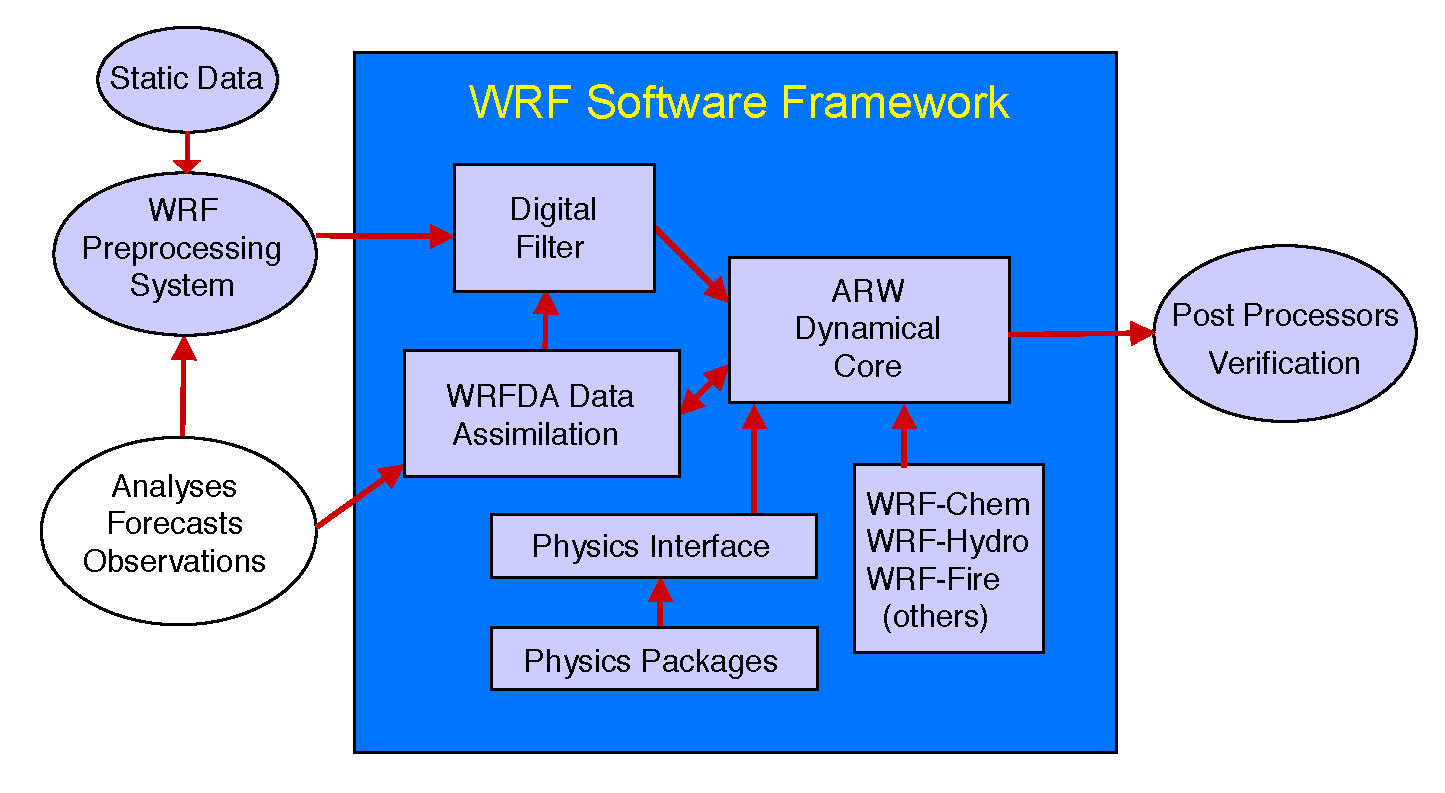
\includegraphics[width=6.5in]{figures/component.pdf}
  \caption{\label{figure:1}WRF system components.}
\end{figure}

\section {Advanced Research WRF (ARW)}

The ARW is a configuration of the WRF system featuring
the ARW dynamics solver together with other compatible components 
to produce a simulation.  Thus, 
it is a subset of the WRF system that, in addition to the specific solver, 
encompasses physics schemes, numerics/dynamics options, 
initialization routines, and a data assimilation package (WRFDA).  
The ARW solver has the WSF in common with the NMM solver and all other 
WRF components within the framework.  While physics packages are 
largely shared by both the ARW and NMM solvers, specific 
compatibility varies with the schemes considered.  
Note that the association of a component of the WRF system with 
the ARW does not preclude the component from being in
WRF configurations that use the NMM solver.  
The following section highlights the major features of the 
ARW Version 4, first released in May 2018.

This technical note focuses on the scientific and algorithmic 
approaches in the ARW, including the solver, physics options,
initialization capabilities, boundary conditions, and grid-nesting techniques.  
The WSF provides the software infrastructure.  
WRFDA, the data assimilation system for WRF, was  
originally adapted from the MM5 
(Pennsylvania State University--NCAR Mesoscale Model 5) 
3DVAR (3-dimensional variational data assimilation) system 
\citep{barker04} and is encompassed within the ARW.
While WRF-Chem and other tailored systems 
(e.g., WRF-Hydro, etc.) use the ARW solver, they are 
not covered by this technical note.  Those seeking details on 
WRF-Chem may consult \citet{Grelletal05} and 
https://ruc.noaa.gov/wrf/wrf-chem/.  Furthermore, for information on 
actually running the ARW system, the ARW Version 4 Modeling System User's Guide 
(http://www2.mmm.ucar.edu/wrf/users/docs/user_guide_V4/WRFUsersGuide.pdf) 
covers model operation. 

\section {Major Features of the ARW System, Version 4}

\vskip 12pt
{\noindent\bf ARW Solver}
\vskip 12pt

\begin{description}
\setlength{\itemsep}{-5pt}
\item{$\bullet$} {\em Equations:}
Fully compressible, Euler nonhydrostatic with 
a run-time hydrostatic option available. Conservative for scalar variables.
%
\item{$\bullet$} {\em Prognostic Variables:}
Velocity components $u$ and $v$ in Cartesian coordinate, vertical velocity $w$, 
perturbation moist potential temperature, perturbation geopotential, 
and perturbation surface pressure of dry air.
Optionally, turbulent kinetic energy and any number of scalars
such as water vapor mixing ratio, rain/snow mixing ratio,
cloud water/ice mixing ratio, and chemical species and tracers.
%
\item{$\bullet$} {\em Vertical Coordinate:}
Terrain-following, mass-based, hybrid sigma-pressure vertical coordinate based on dry hydrostatic presure, 
with vertical grid stretching permitted.
Top of the model is a constant pressure surface.
%
\item{$\bullet$} {\em Horizontal Grid:}
Arakawa C-grid staggering. 
%
\item{$\bullet$} {\em Time Integration:}
Time-split integration using a 2nd- or 3rd-order Runge-Kutta scheme with
smaller time step for acoustic and gravity-wave modes. 
Variable time step capability.
%
\item{$\bullet$} {\em Spatial Discretization:}
2nd- to 6th-order advection options in horizontal and vertical.
%
\item{$\bullet$} {\em Turbulent Mixing and Model Filters:} Sub-grid scale
turbulence formulation in both coordinate and physical space.
Divergence damping, external-mode filtering, vertically implicit
acoustic step off-centering. Explicit filter option.
%
\item{$\bullet$} {\em Initial Conditions:}
Three dimensional for real-data, and one-, two- and 
three-dimensional for idealized data. 
Digital filtering initialization (DFI) capability 
available (real-data cases).
%
\item{$\bullet$} {\em Lateral Boundary Conditions:} 
Periodic, open, symmetric, and specified options available.
%
\item{$\bullet$} {\em Top Boundary Conditions:} 
Gravity wave absorbing (diffusion, Rayleigh damping, or implicit 
Rayleigh damping for vertical velocity).  
Constant pressure level at top boundary along a material surface. 
Rigid lid option.
%
\item{$\bullet$} {\em Bottom Boundary Conditions:} 
Physical or free-slip.
%
\item{$\bullet$} {\em Earth's Rotation:}
Full Coriolis terms included.
%
\item{$\bullet$} {\em Mapping to Sphere:} 
Four map projections are supported for real-data simulation: 
polar stereographic, Lambert conformal, Mercator, and 
latitude-longitude (allowing rotated pole). 
Curvature terms included.
%
\item{$\bullet$} {\em Nesting:} 
One-way interactive, two-way interactive, and moving nests.
Multiple levels and integer ratios.
%
\item{$\bullet$} {\em Nudging:}
Grid (analysis) and observation nudging capabilities available. 
%
\item{$\bullet$} {\em Global Grid:}
Global simulation capability using polar Fourier filter and 
periodic east-west conditions. 
\end{description}

\newpage
\vskip 12pt
{\noindent\bf Model Physics}
\vskip 12pt

\begin{description}
\setlength{\itemsep}{-5pt}
\item{$\bullet$} {\em Microphysics:} Schemes ranging from simplified
physics suitable for idealized studies to mixed-phase, multi-moment, and aerosol-aware
approaches to support process studies and accurate NWP.
%
\item{$\bullet$} {\em Cumulus parameterizations:}
Adjustment, mass-flux, and scale-aware schemes available.
%
\item{$\bullet$} {\em Surface physics:}
Multi-layer land surface models ranging from a simple thermal model to full
vegetation and soil moisture models, including snow cover and sea ice.
%
\item{$\bullet$} {\em Planetary boundary layer physics:}
Turbulent kinetic energy prediction or non-local $K$ schemes.
%
\item{$\bullet$} {\em Atmospheric radiation physics:} 
Longwave and shortwave schemes with multiple spectral bands and a 
simple shortwave scheme suitable for climate and weather applications.  
Cloud effects and surface fluxes are included.
\end{description}

\vskip 12pt
{\noindent\bf WRFDA System}
\vskip 12pt

\begin{description}
\setlength{\itemsep}{-5pt}
\item{$\bullet$} Data assimilation capability merged into WRF software framework.
%
\item{$\bullet$} Incremental formulation of the model-space cost function.
%
\item{$\bullet$} Quasi-Newton or conjugate gradient minimization algorithms.
%
\item{$\bullet$} Analysis increments on unstaggered Arakawa-A grid.
%
\item{$\bullet$} Representation of the horizontal component of background 
error ${\bf B}$ via recursive filters (regional) or power spectra (global). The
vertical component is applied through projection onto climatologically-averaged 
eigenvectors of vertical error. Horizontal/vertical errors are
non-separable (horizontal scales vary with vertical eigenvector).
%
\item{$\bullet$}  Background cost function ($J_b$) preconditioning 
via a control variable transform ${\rm U}$ defined as ${\bf B}={\rm U} {\rm U}^T$.
%
\item{$\bullet$} Flexible choice of background error model and control variables.
%
\item{$\bullet$} Background error covariances estimated via either the
NMC-method of averaged forecast differences or suitably-averaged
ensemble perturbations.
%
\item{$\bullet$} 3DVAR, 4DVAR, hybrid ensemble-3DVAR approaches available. 
Global and regional, multi-model DA capability.
%
\end{description}

\vskip 12pt
{\noindent\bf WRF-Chem}
\vskip 12pt

\begin{description}
\setlength{\itemsep}{-5pt}
\item{$\bullet$} Online (or ``inline'') model, in which the model is consistent
with all conservative transport done by the meteorology model. 
%
\item{$\bullet$} Dry deposition, coupled with the soil/vegetation scheme.
%
\item{$\bullet$} Aqueous phase chemistry coupled to some of the microphysics and aerosol schemes.
%
\item{$\bullet$} Three choices for biogenic emissions:
No biogenic emissions; Online calculation of biogenic emissions; Online modification 
of user specified biogenic emissions (e.g., EPA Biogenic Emissions Inventory System (BEIS)).
%
\item{$\bullet$} Two choices for anthropogenic emissions:
No anthropogenic emissions and user-specified anthropogenic emissions.
%
\item{$\bullet$} Two choices for gas-phase chemical reaction calculations:
RADM2 chemical mechanism and CBM-Z mechanism.
%
\item{$\bullet$} Several choices for gas-phase chemical reaction calculations 
through the use of the Kinetic Pre-Processor (KPP). 
%
\item{$\bullet$} Three choices for photolysis schemes:
Madronich scheme coupled with hydrometeors, aerosols, and convective parameterizations;
Fast-J Photolysis scheme coupled with hydrometeors, aerosols, and convective parameterizations;
FTUV scheme scheme coupled with hydrometeors, aerosols, and convective parameterizations.
%
\item{$\bullet$} Choices for aerosol schemes:
The Modal Aerosol Dynamics Model for Europe (MADE/SORGAM);
Model for Simulating Aerosol Interactions and Chemistry (MOSAIC); and 
The GOCART aerosol model (experimental). 
%
\item{$\bullet$} A tracer transport option in which the chemical mechanism, 
deposition, etc., has been turned off. 
\end{description}

\vskip 12pt
{\noindent\bf WRF Software Framework}
\vskip 12pt

\begin{description}
\setlength{\itemsep}{-5pt}
\item{$\bullet$} Highly modular, single-source code for maintainability.
%
\item{$\bullet$} Two-level domain decomposition for parallel and 
shared-memory generality.
%
\item{$\bullet$} Portable across a range of available computing platforms.
%
\item{$\bullet$} Support for multiple dynamics solvers and physics modules.
%
\item{$\bullet$}
Separation of scientific codes from parallelization and other 
architecture-specific aspects.
%
\item{$\bullet$}
Input/output Application Program Interface (API) enabling various external
packages to be installed with WRF, thus allowing WRF
to easily support various data formats.
%
\item{$\bullet$}
Efficient execution on a range of computing platforms
(distributed and shared memory, vector
and scalar types). Support for accelerators (e.g., GPUs).
%
\item{$\bullet$}
Use of Earth System Modeling Framework (ESMF) and interoperable as an ESMF
component.
%
\item{$\bullet$}
Model coupling API enabling WRF to be coupled with other models such as
ocean, and land models using ESMF, MCT, or MCEL.
\end{description}
